\documentclass[]{article}
\usepackage[utf8]{inputenc}
\usepackage[danish,english]{babel}
\usepackage{graphicx}
\usepackage[usenames]{xcolor}
\usepackage{times}
\usepackage{listings}
\usepackage{textcomp}
\usepackage{hyperref}
\usepackage{textpos}
\usepackage{pgfgantt}
\usepackage{lscape}
\usepackage{indentfirst}
\usepackage{tikz}
\usepackage{pgfplots}
\usepackage{ifthen}
\usepackage{float}
\usepackage{pict2e}
\usepackage[export]{adjustbox}
\pgfplotsset{compat=1.13}
\usepackage{siunitx}
\usepackage{tabularx}

% adjustment to page format
\marginparwidth=0pt
\oddsidemargin=0pt
%\evensidemargin=0pt
\marginparsep=0pt
%\topmargin=-15 mm
\textwidth=168 mm
\textheight=210 mm
\parskip 0.27 em
\parindent=0pt
%\leftmargin=1cm
\pagenumbering{arabic}
% Define DTU color
\definecolor{dtured}{RGB}{153,0,0}
\title{Projektplan}

\begin{document}
% formel header
\thispagestyle{empty}
\vspace*{-1.9cm}
\begin{textblock*}{18cm}[0,0](0cm,-2cm) %
  \noindent
  
\includegraphics[width=6.5cm,valign=t]{documentation/resources/Stor-mobil-top_DTU_Elektro_UK.png}
  \hspace*{8.6cm}
  
\includegraphics[width=1.5cm,valign=t]{documentation/resources/tex_dtu_logo.pdf}
\end{textblock*}
\begin{textblock*}{19.0cm}(0cm,-2.5cm) %
\begin{center}
  {\color{dtured}\large31015 Introductory project}\\
  \normalsize
  s186083 Tjark Petersen\\
  s194006 Steffan Martin Kunoy\\
  s194027 Victor Alexander Hansen\\
\end{center}
\end{textblock*}
% rød streg
\vspace{1mm}
{\hspace*{-0.1cm}
\color{dtured}\noindent \rule{16.8cm}{5pt}}

 
\begin{table}[H]
     \centering
     \begin{tabularx}{\textwidth}{|X|X|X|}
     \hline
          DTU Electro&Spring 2021 & Group: 7, ID: MEK2 \\\hline
          Course 31015 & Title & Group members \\\hline
          Introductory project - Electrotechnology & ROAST Telemetry & \begin{tabular}{l} s186083 Tjark Petersen\\s194006 Steffan Martin Kunoy\\s194027 Victor Alexander Hansen \end{tabular}\\\hline
          Document:& Project plan & 4 pages\\\hline 
          Version/Status: & 1. edition &\today\\\hline
     \end{tabularx}
 \end{table}
 
\section{Problem introduction}

This project concerns a telemetry module for use by the DTU Roadrunners Solar Team (ROAST). In 2023, ROAST is set to participate in the Bridgestone World Solar Challenge, a race spanning over 3000 km across Australia from Darwin in Northern Territory to Adelaide in South Australia. The solar car have limited opportunities for recharging during the race, so the main source of energy during the race, is from solar energy. To this end, solar panels will cover the car, however, the solar car is only allowed to have a maximum of 4 square meters of solar panels. This emphasizes the need to create an energy-efficient solar car to win the race \cite{wsc}.\\
%Dette projekt vil omhandle et telemetri modul som skal indgå i DTU Roadrunners Solar Team (ROAST). I 2023 deltager ROAST i Bridgestone World Solar Challenge, som er et løb på over 3000 km tværs gennem Australien \cite{wsc}. Den primære energikilde for bilen under løbet er derfor solenergi.\\
\\
Throughout the race the solar car will be monitored by a support car, which can monitor the car's condition and issue commands. This is a crucial function as the solar car will be navigating Australia's busy highways, where the heat and tire pressure may cause a detriment to the vehicle. The support car will therefore be able to analyze and react to the data stream being transmitted from the solar car, even when the driver is preoccupied by driving the car and navigating traffic. \\
%I løbet vil solbilen være ledsaget af en følgebil, som skal overvåge solbilens driftstatus og sende kommandoer til solbilen. Dette er en yderst vigtig opgave, da bilerne skal køre tværs gennem Australien i offentlig trafik, hvor alt fra varme til dæktryk udfordrer solbilen. Følgebilen vil derfor have mulighed for at analysere og reagere på data fra solbilen, hvis køreren i solbilen er optaget af trafik og betjening af solbilen.
\\
The main function of the telemetry module is to read data from the solar car's on-board CAN (Controller Area Network) bus and transmit it via an RF-transceiver to the support car, while simultaneously logging data locally in a "black box" memory chip. The support car is equipped with a similar module such that the support crew can react to the data manually or automatically by sending commands back to the CAN bus. As a consequence, the telemetry module plays a vital role in the communication between both vehicles, considering the distance between them may be up to 1 km depending on traffic conditions.\\
%Telemetri modulets opgave er at aflæse sensordata fra solbilens CAN (Controller Area Network) bus og sende dataen via en RF-transceiver til følgebilen såvel som at logge dataen lokalt i et "black box" hukommelseschip. Et lignende modul skal også være til stede i følgebilen, så følgebilen omvendt kan reagere på denne data, enten automatisk eller ved menneskelig ageren, og sende kommandoer tilbage til solbilens CAN bus. Telemetri modulet spiller derfor en afgørende rolle, da man også skal tage højde for at afstanden mellem solbil og følgebil kan være op til 1 km alt afhængig af trafikforholdene.
\\
Therefore, the telemetry module must both serve the purpose of fulfilling the necessary specifications for communication, while also being as energy-efficient as possible. The project will mainly focus on the former that is, ensuring that the module meets the specifications with a solid solution.

\section{Problem description}
Remote sensing of data from the solar car will give the ROAST team a competitive advantage as the support vehicle will take on a more active role in controlling and optimising the car's performance. This will ease the burden on the driver and engage a large part of the supporting crew. For these reasons we have chosen to focus our project on the following points:   
%Fjernmåling af data fra solbilen vil give ROAST en fordel i og med at support bilen kan indtage en mere aktiv rolle i styring og optimering af bilen. Det letter derfor på kørerens arbejdsbyrde, og fordeler ansvaret for hele ROAST-support holdet. Af denne grund vil vi afgrænse projektet på følgende punkter: 
\begin{itemize}
    \item How can we design a module that can read and write sensor data and commands from a CAN bus network? 
    %\item Hvordan kan vi lave et modul der kan læse, sende og modtage sensor data og kommandoer i CAN bus netværket?
    \item How can CAN data be transmitted over a distance of up to one kilometer? 
    %\item Hvordan kan CAN data overføres trådløst i en afstand på en kilometer?
    \item How does the support-car module process data upon receiving it from the solar car?
    %\item Hvordan skal data behandles ved modtagelse i følgebilen?
    \item What is the best method for storing data locally (black box) while being accesible at a later time? 
    %\item Hvordan kan data bedst gemmes lokalt (black box) og udlæses på et senere tidspunkt?
\end{itemize}

\section{Problem scope}

There are multiple solutions to the problem at hand that were discussed, among them implementing a whole solution on a PCB or more modular solutions involving prebuild microcontrollers like the Teensy\cite{teensy}. We chose to consider prebuild microcontroller based solutions and to not focus on implementing the final product on a PCB. The decision was based on us wanting to design a product which is modular and flexible and thus can be altered and improved during its life time.\\
\\
A PCB implementation is expected to achieve a higher efficiency due to reduced current draw compared to the implementations we are considering. We prioritized a more modular and flexible product over the potential power savings though since the difference in current draw is expected to be of the order of some tenths of milli-Ampère.

%Vi har i vores gruppe diskuteret flere forskellige umiddelbare løsningsformer for projektets produkt, heriblandt at lave en løsning på et PCB board, eller en løsning på et Teensy board/FPGA board. Vi har valgt at afgrænse os til at se på Teensy og FPGA løsninger, og ikke PCB boards. Dette skyldes at det hardware design vi kommer frem til som produkt kan redigeres mere fleksibelt undervejs på et Teensy og FPGA board, fremfor et PCB board som er mere special designet til formålet.\\
%\\
%Det skal dog siges at vi forventer at et PCB board design ville være mindre strømkrævende end de løsninger vi ser på, men vi har i dette projekt valgt at prioritere et godt design over strømbesparelse, siden der formentlig er tale om forskel i størrelsesorden af nogen tiende af mA.
\section{Target audience}
The target audience for our project is the DTU ROAST team, who will integrate the telemetry module in the solar car and support vehicle. Subsequently, the car is set to enter the 2023 Bridgestone World Solar Challenge.

\section{Problem solution}
\begin{enumerate}
    \item Preliminary design of telemetry module in block diagram form. Establish specifications and requirements for the final product. 
    %\item Foreløbigt design af telemetrimodulet som blokdiagram. Fastslå specifikationer og krav til løsningen. 
    \item Select components for preliminary design. Ordering components not available from DTU. 
    %\item Valg af komponenter til det indledende design. Bestilling af komponenter som ikke kan fremskaffes på DTU. 
    \item Prototyping telemetry module on two breadboards. Write code to test limited functionality. 
    %\item Første prototype af telemetrimodul på breadboard. Skrive kode til at teste begrænset funktionalitet. 
    \item Improve on prototype. Order new components if needed. Optimize code and write more extensive tests. 
    %\item Foreslå forbedringer til første prototype. evt. bestille nye komponenter. Optimer kode og design mere omfattende tests.
    \item Improved prototype of telemetry module on breadboard. Repeat Steps 3. and 4. until fundamental requirements in Step 1. are satisfied. 
    %\item Anden prototype af telemetrimodul på breadboard. Gentag 3. og 4. indtil grundlæggende krav i 1. er opfyldt. 
    \item Develop more permanent solution, i.e. compact, soldered and configurable. Complete tests in Step 5.
    %\item Udvikle mere færdig løsning, dvs. kompakt, loddet og programmerbar. Gennemfør tests som i 5.
    \item Design GUI for interaction with PC. Test with USB connection to support-car module. Remote control via PC. 
    %\item Design af GUI til interaktion med PC. Test med USB forbindelse til support-bil modul. Styring via PC.  
    \item Present solution to DTU ROAST team. Discuss improvements and additional features. 
    %\item Præsenter løsning for DTU ROAST holdet. Diskuter forbedringer og features. 
    \item Integrate telemetry module with solar car. Ongoing testing of solution. Feedback and evaluate project. 
    %\item Integration med solbil, løbende tests og evaluering af projekt. 
\end{enumerate}
\section{Resources}
\begin{itemize}
    \item 1x Teensy 4.0 development board
    \item 1x Teensy 4.1 development board
    \item 2x nRF24L01 + PA/LNA Wireless Transceiver with antenna
    \item 1x Micro SD memory card (32GB)
    \item 2x MCP2551 CAN Transceiver w/ breakout board
\end{itemize}
At this stage, our telemetry modules, one for both the solar and support car, will consist of the components above. The size of the memory SD card is uncertain at this point, but we will use 32GB for testing purposes.\\
\\
In addition to the hardware ressources needed for this project, the DTU ROAST team provides a great source of insight for the project. Reports from different teams and last years telemetry project lies available, which helps laying the groundwork for our project \cite{ROAST}.

\section{Activity Plan}
\begin{figure}[H]
    \centering
    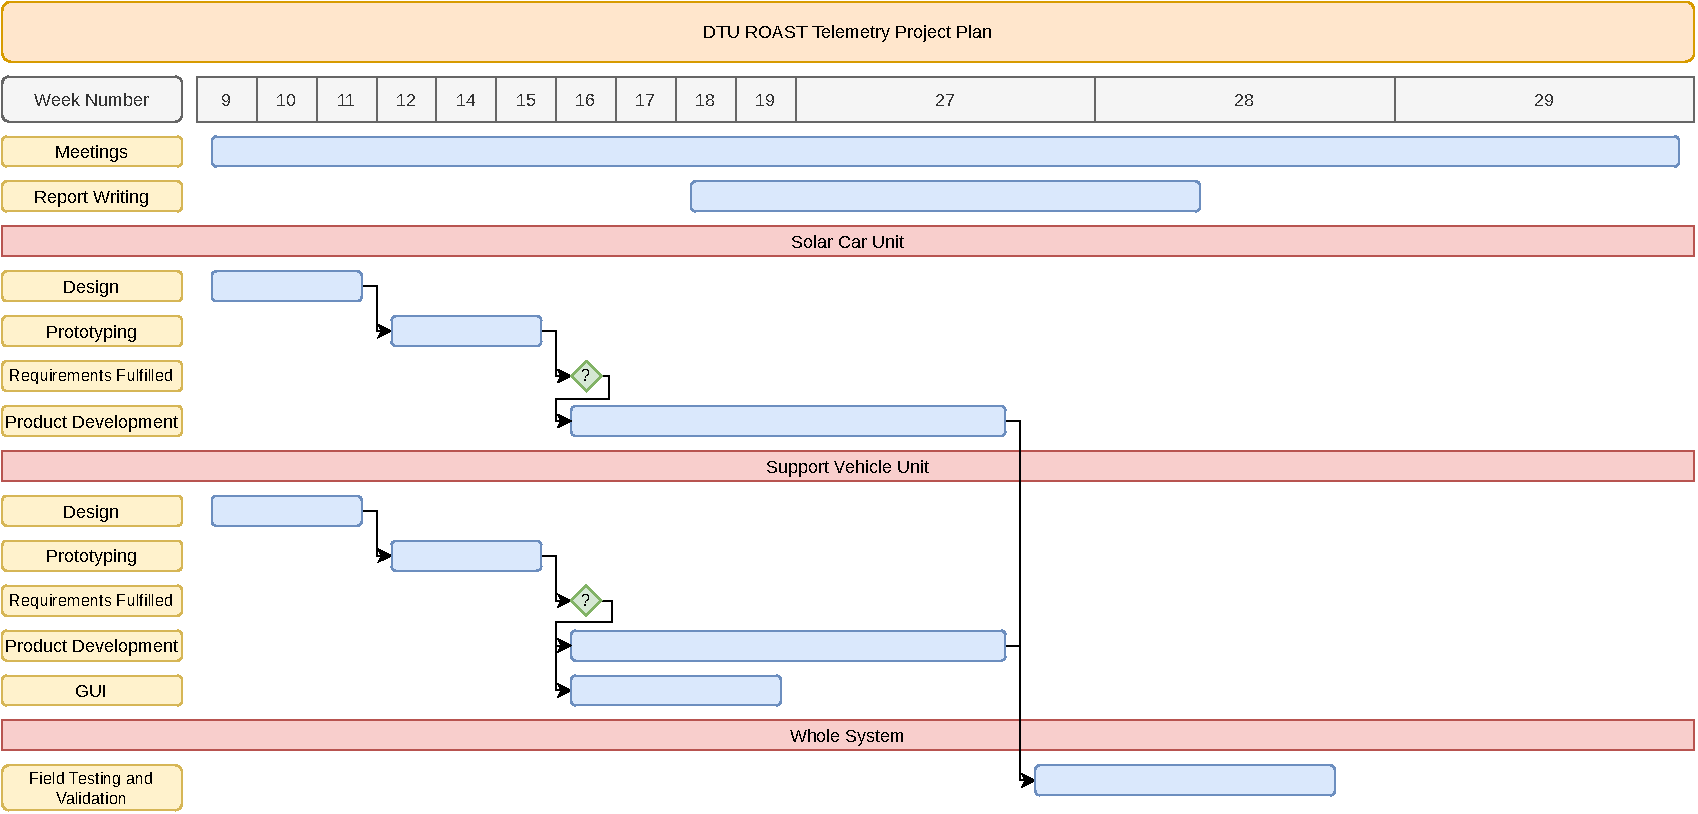
\includegraphics[width=\textwidth]{documentation/images/projectPlan.pdf}
    \caption{The project activity plan}
    \label{fig:my_label}
\end{figure}
\subsection*{Meetings}
We will have a weekly meeting with both the project coordinator Christian Kampp Kruuse and our supervisor Martin Schoeberl on Fridays. In addition, meetings will be arranged with our second supervisor Vitaliy Zhurbenko if necessary. 
\subsection*{Report writing}
We will begin drafting a project report once we have achieved an MVP (Minimum Viable Product). The report will include full documentation of all design choices in hardware and software. 
\subsection*{Design}
The design phase of the project will include designing prototypes to be implemented once the hardware components become available. Furthermore, basic software programs may be written and debugged during the design phase. We intend for all design, prototyping and testing of the Solar Car Unit (SC) and Support Vehicle Unit (SV) to run in parallel. 
\subsection*{Prototyping}
During prototyping we want to test the basic functionality of our product. The setup should be configurable, which is why we plan to use breadboards and jumper wires. Basic tests will be written in software to make sure the product meets the basic requirements. 
\subsection*{Requirements fulfilled}
Once the basic requirements have been fulfilled by the prototype we will begin rigorously testing to find ways to further optimise our design. This is to ensure that the product will not have any fundamental flaws. 
\subsection*{Product Development}
This stage will concern the design of an MVP as well as later design iterations. 
\subsection*{GUI}
As a final touch we intend to create a basic GUI allowing PC users to interact with the telemetry module, as well as sending and receiving data on the CAN bus. 
\subsection*{Field Testing and Validation}
Finally, our product will be integrated with the ROAST solar car and support vehicle, allowing us to test it in operation. We will be able to gain feedback from the DTU ROAST team and evaluate the project. 
\newpage
\section{System Specification}

In the following three subsections feature lists for each of the three systems are presented.

\subsection{Solar Car Unit (SC)}
\begin{table}[H]
    \centering
    \begin{tabular}{|l|l|}
    \hline
        \textbf{Feature ID} & \textbf{Description} \\ \hline
        \textbf{SC.SD} & The system uses a SD card as a permanent storage of log files \\ \hline
        SC.SD.write & Write a data structure to a file on the SD card \\ \hline
        SC.SD.read & Read a file into a data structure \\ \hline
         &  \\ \hline
        \textbf{SC.RF} & The system needs to communicate via a RF module with the support vehicle \\ \hline
        SC.RF.rxCmd & Receive a system configuration command from the support vehicle \\ \hline
        SC.RF.rxCanCmd & Receive a message to be broadcasted via the solar car CAN bus \\ \hline
        SC.RF.txResp & Transmit response to a received command \\ \hline
        SC.RF.txLogUnit & Transmit a log unit to the support vehicle \\ \hline
        SC.RF.txLogFile & Transmit a log file to the support vehicle \\ \hline
         &  \\ \hline
        \textbf{SC.CAN} & The system needs to communicate via the solar car CAN bus \\ \hline
        SC.CAN.rx & Receive all messages broadcasted on the CAN bus \\ \hline
        SC.CAN.tx & Transmit a message on the CAN bus \\ \hline
         &  \\ \hline
        \textbf{SC.BUF} & The system needs to buffer logged data in local flash memory until enough data to fill a file is collected \\ \hline
        SC.BUF.add & Add a log unit to the buffer \\ \hline
        SC.BUF.rd & Read a logging unit from the buffer into RAM \\ \hline
        SC.BUF.rdToFile & Read all logged data from the buffer into a file \\ \hline
        SC.BUF.clr & Empty the buffer \\ \hline
    \end{tabular}
\end{table}

\subsection{Support Vehicle Unit (SV)}
\begin{table}[H]
    \centering
    \begin{tabular}{|l|l|}
    \hline
        \textbf{Feature ID} & \textbf{Description} \\ \hline
        \textbf{SV.RF} & The system needs to communicate via RF with the solar car \\ \hline
        SV.RF.txCmd & Transmit a system configuration command to the solar car \\ \hline
        SV.RF.txCanCmd & Transmit a CAN message to the solar car \\ \hline
        SV.RF.rxResp & Receive a response from the solar car unit \\ \hline
        SV.RF.rxLogUnit & Receive a log unit from the solar car unit \\ \hline
        SV.RF.rxLogFile & Receive a log file from the solar car unit \\ \hline
         &  \\ \hline
        \textbf{SV.UART} & The system needs to communicate with a computer via UART \\ \hline
        SV.UART.rxCmd & Receive a command via UART \\ \hline
        SV.UART.rxCanCmd & Receive a CAN bus message via UART \\ \hline
        SV.UART.txLogUnit & Transmit a log unit to the computer \\ \hline
        SV.UART.txLogFile & Transmit a log file to the computer \\ \hline
    \end{tabular}
\end{table}

\subsection{Support Vehicle Computer Program (PR)}
\begin{table}[H]
    \centering
    \begin{tabular}{|l|l|}
    \hline
        \textbf{Feature ID} & \textbf{Description} \\ \hline
        \textbf{PR.UART} & The program needs to communicate with the support vehicle unit via UART \\ \hline
        PR.UART.txCmd & Transmit a system configuration command via UART \\ \hline
        PR.UART.txCanCmd & Transmit a CAN message via UART \\ \hline
        PR.UART.rxLogUnit & Receive a log unit via UART \\ \hline
        PR.UART.rxLogFile & Receive a log file via UART \\ \hline
         &  \\ \hline
        \textbf{PR.FILE} & The program needs to output received log files \\ \hline
        PR.FILE.write & Write a file containing the last received log file \\ \hline
         &  \\ \hline
        \textbf{PR.GUI} & The program is interface via a GUI \\ \hline
        PR.GUI.getConf & Get configuration parameters from GUI \\ \hline
        PR.GUI.getCanCmd & Get a CAN message from the GUI \\ \hline
        PR.GUI.monitor & Show incoming log data stream \\ \hline
        PR.GUI.saveLog & Pass log file to file writer \\ \hline
    \end{tabular}
\end{table}

\section{References}
\begingroup
\renewcommand{\section}[2]{}%
%\renewcommand{\chapter}[2]{}% for other classes
\begin{thebibliography}{}
\bibitem{wsc}
Bridgestone World Solar Challenge, 
URL: https://worldsolarchallenge.org/
\bibitem{ROAST}
Reports and source files provided by DTU ROAST
\bibitem{teensy}
Teensy microcontroller,
URL: https://www.pjrc.com/teensy/
\end{thebibliography}
\endgroup

\end{document}